\clearpage
\subsection{Program} % (fold)
\label{sub:program}

In most software projects the top level \emph{artefact} you are aiming to create is a \textbf{program}. Within your software a program is a list of instructions the computer will perform when that program is run on the computer.

When you create a program in your code you should be thinking about the tasks you want the program to achieve, and the steps you must get the computer to perform when the program is run. These then become the instructions within the program, with each instruction being a \nameref{sub:statement} of what you want performed.

\begin{figure}[h]
   \centering
   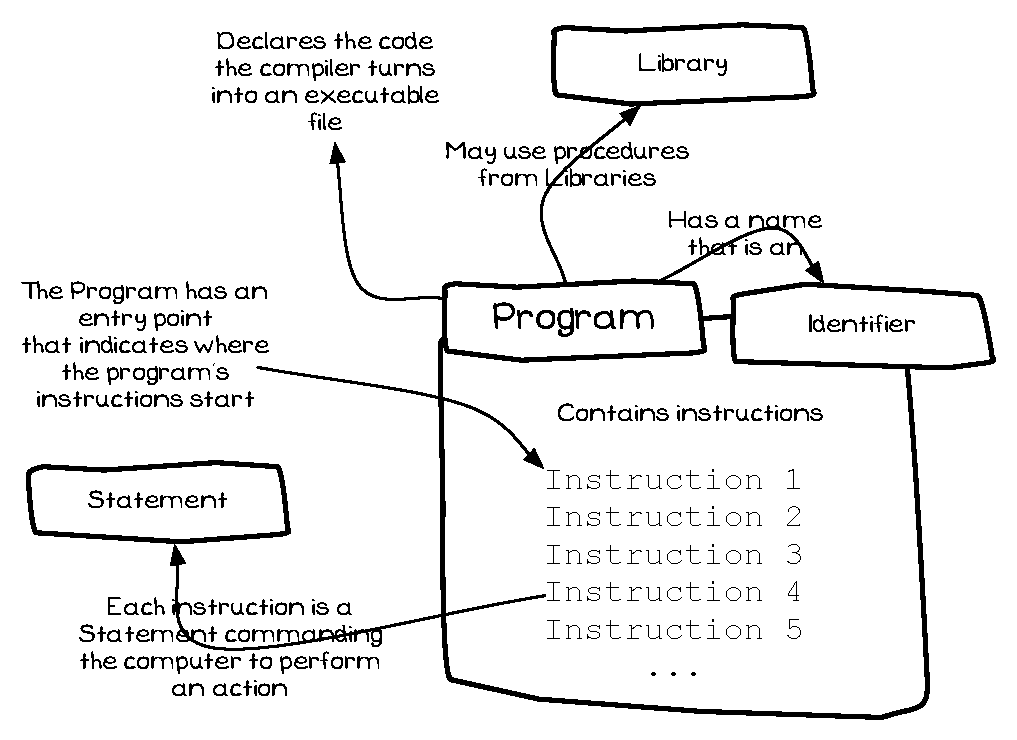
\includegraphics[width=\textwidth]{./topics/program-creation/diagrams/BasicProgramConcept} 
   \caption{A program contains instructions that command the computer to perform actions}
   \label{fig:program-creation-program}
\end{figure}


\mynote{
\begin{itemize}
  \item A program is an \textbf{artefact}, something you can create in your code.
  \item Figure \ref{fig:program-creation-program} shows the concepts related to the program's code.
  \item A program is a programming artefact used to define the steps to perform when the program is run.
  \item You use a compiler to convert the program's source code into an executable file.
  \item By declaring a program in your code you are telling the compiler to create a file the user can run (execute).
  \item The program has an \textbf{entry point} that indicates where the program's instructions start.
  \item The name of the program determines the name of the executable file.
  \item Your program can use code from a \nameref{sub:library} or number of libraries.
  \item In programming terminology, an instruction is called a \nameref{sub:statement}.
\end{itemize}
}

% section program (end)